\documentclass[conference]{IEEEtran}

\usepackage{graphicx}
\usepackage{amsmath}
\usepackage{enumitem}
\usepackage{float}
\usepackage[T1]{fontenc}

\title{EE599 Research Project\\3. Device Design and Implementation}

\author{
\IEEEauthorblockN{Hari Krishna Koneti}
\IEEEauthorblockA{
M.S. Electrical Engineering
}
}

\begin{document}

\maketitle

\section{Device Design and Implementation}

PostureSense is a wearable concept based on Arduino Uno R3 and Spark Fun ADXL345 
to distinguish between sleep positions (supine, prone, left, right). The design is simple, 
inexpensive, and dependable..

\subsection{Hardware Design}

Arduino Uno R3 performs acquisition and classification. ADXL345 measures 3-axis 
acceleration. System is powered via USB from laptop for development.

\subsection{Electrical Connections and Schematic}

I2C connections: SDA$\to$A4, SCL$\to$A5, VCC$\to$3.3V, GND$\to$GND.

\begin{figure}[!t]
    \centering
    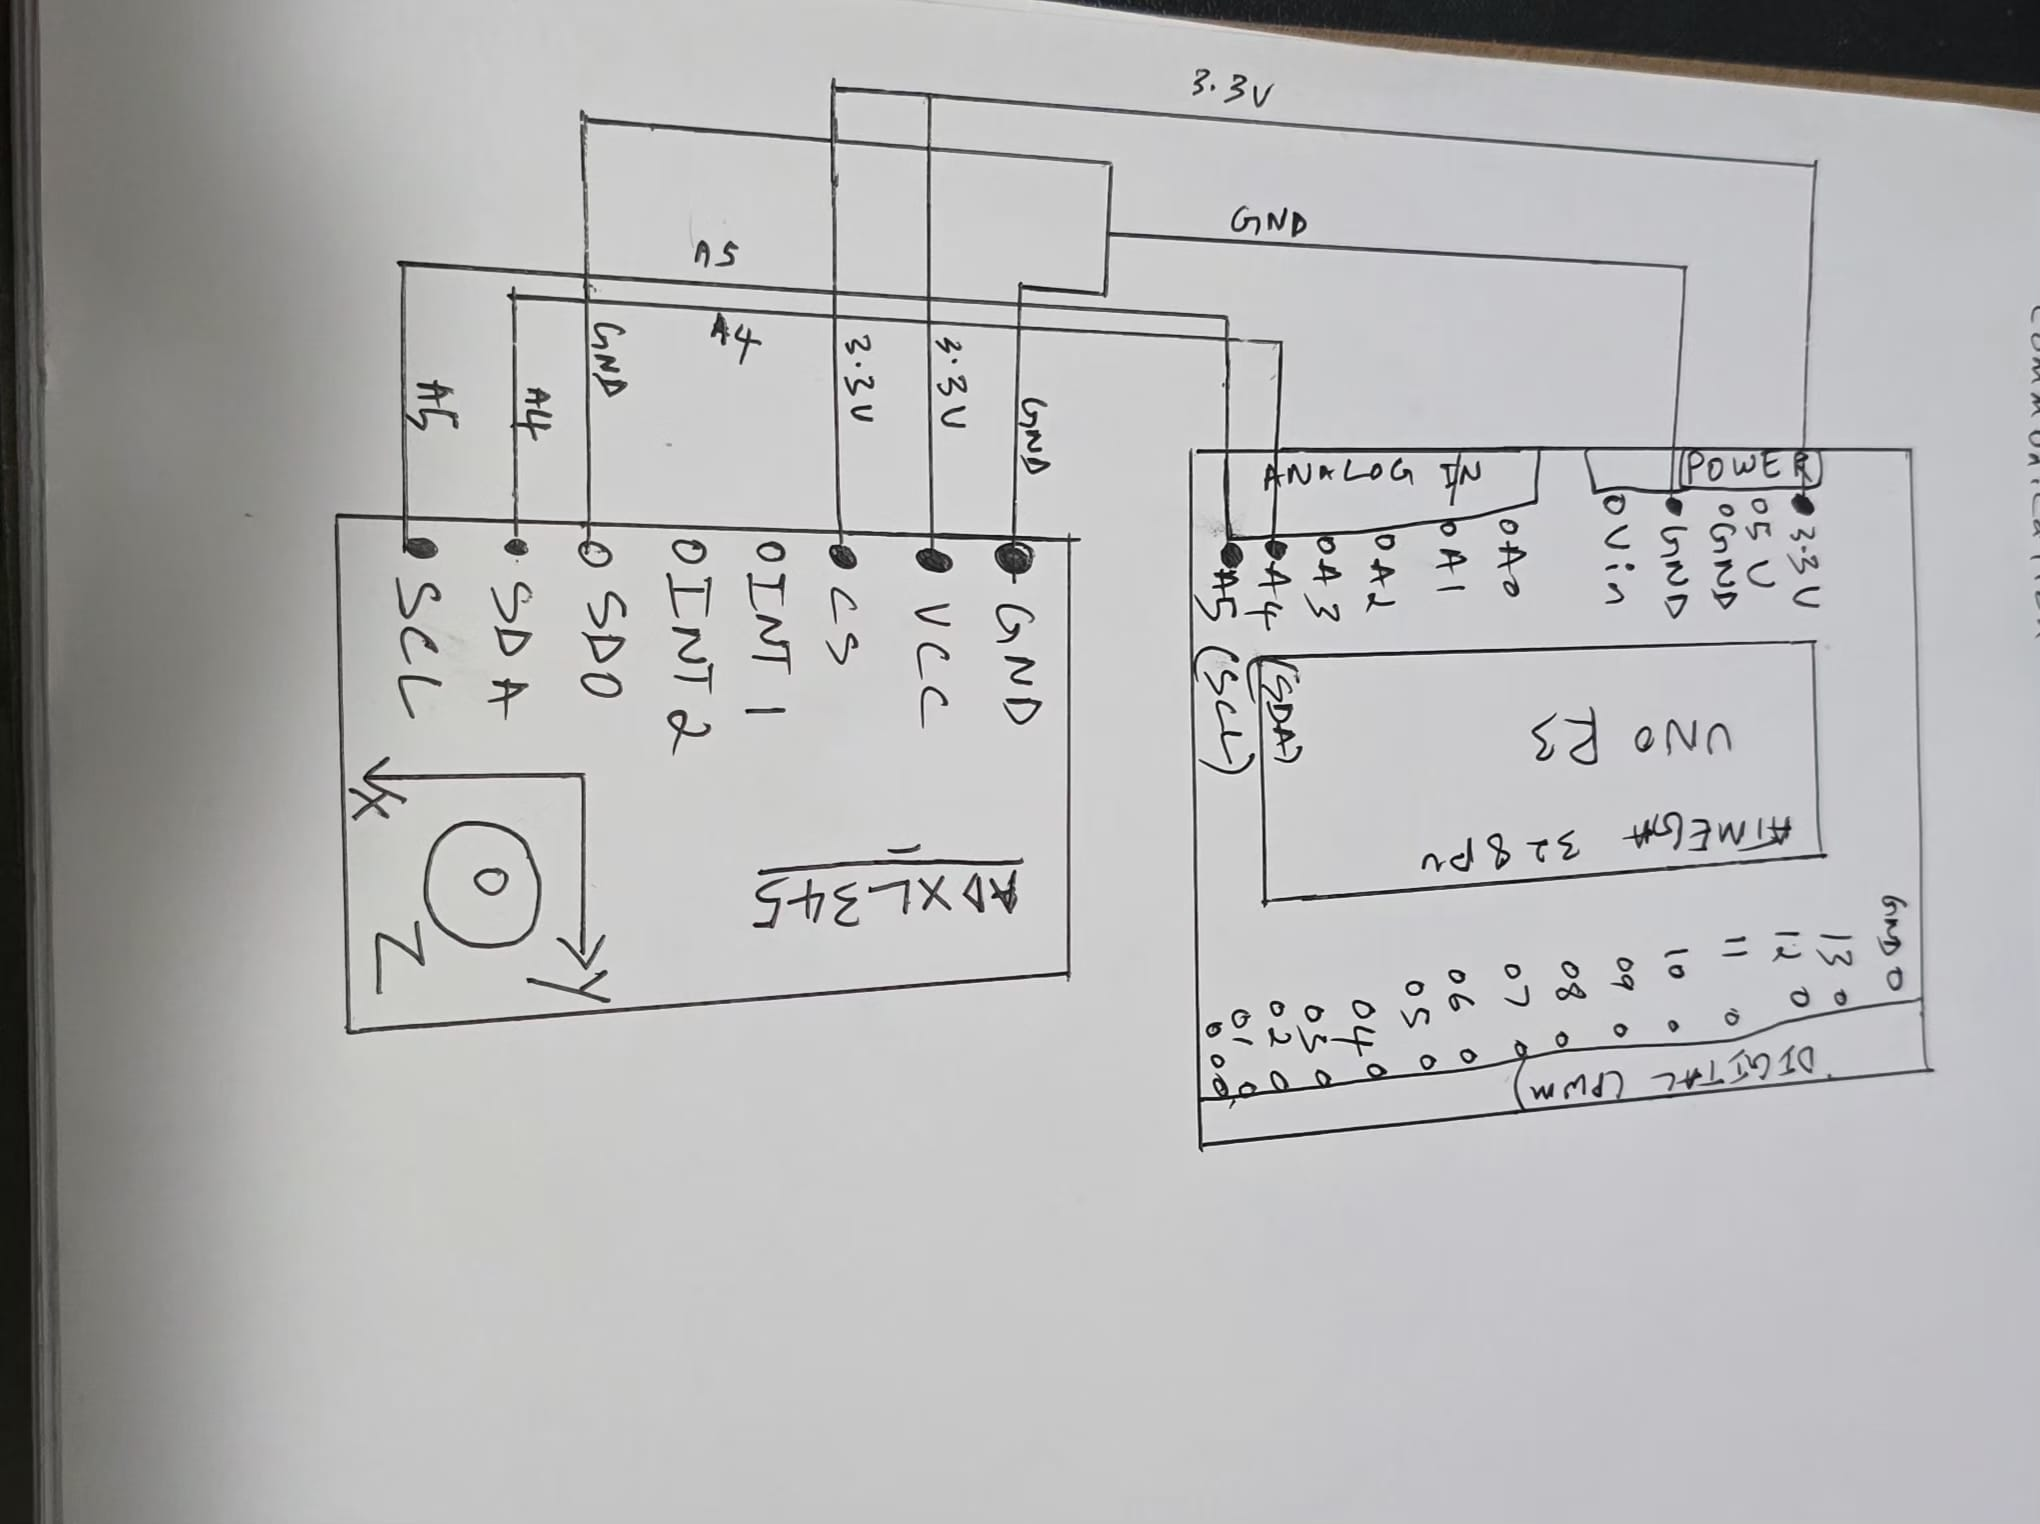
\includegraphics[width=0.95\columnwidth]{Electrical Connections and Schematic.jpeg}
    \caption{Hand-drawn electrical schematic showing the Arduino Uno R3 connected to the ADXL345 sensor using I2C communication. The SDA and SCL lines are connected to A4 and A5, respectively, while 3.3V and GND provide power and reference.}
    \label{fig:schematic_handdrawn}
\end{figure}

I2C connections: SDA$\to$A4, SCL$\to$A5, VCC$\to$3.3V, GND$\to$GND.

\subsection{Pin Description and Circuit Explanation}

The Arduino Uno R3 and SparkFun ADXL345 are connected using the I2C 
communication interface. Each pin in the circuit serves a specific role in ensuring proper 
data transmission and power delivery.

\subsubsection{Pin-Level Description}

\textit{ADXL345 Pins}

\begin{itemize}[leftmargin=*,noitemsep]
    \item \textbf{VCC (3.3V)}  
    Sources the ADXL345 sensor. The sensor is powered by 3.3V and feeding it with 
    more power (e.g., 5V), will cause the sensor to break. This pin is tied up to the 
    3.3V output of the Arduino.

    \item \textbf{GND (Ground)}  
    Gives a point of reference to the voltages in the circuit. It gets attached to the 
    Arduino GND to complete the circuit.

    \item \textbf{SDA (Serial Data Line)}  
    Transfers information in both directions between the Arduino and the ADXL345. 
    It is linked to the Analog Pin A4 of Arduino, the SDA line of I2C communication.

    \item \textbf{SCL (Serial Clock Line)}  
    Delays the clock signal that is used to synchronize data exchange between the 
    Arduino (master) and ADXL345 (slave). It is tied to Analog Pin A5 on the 
    Arduino.
\end{itemize}

\textit{Arduino Uno R3 Pins}

\begin{itemize}[leftmargin=*,noitemsep]
    \item \textbf{A4 (SDA)}  
    Used in the I2C data communication. It sends and receives information to/from 
    the ADXL345.

    \item \textbf{A5 (SCL)}  
    Used for I2C clock generation. The Arduino is the master and determines the 
    communication time.

    \item \textbf{3.3V Pin}  
    The output of the ADXL345 sensor is controlled by supplies to 3.3 V.

    \item \textbf{GND Pin}  
    Provides a common ground between the sensor and the Arduino.

    \item \textbf{USB Port (Power Source)}  
    Power the Arduino directly off the laptop and also allows serial access to sensor 
    data monitoring.
\end{itemize}

\subsubsection{Circuit Operation}

\begin{itemize}[leftmargin=*,noitemsep]
    \item The Arduino Uno will be the I2C master and the ADXL345 will be a slave device. 
    The two communicates via the SDA and SCL lines.

    \item The Arduino opens the I2C interface and sets the ADXL345 with SparkFun library.

    \item Arduino transmits instructions to the SDA line which are synchronized by the SCL 
    clock signal.

    \item The ADXL345 then reacts by sending acceleration data ($a_x$, $a_y$ and $a_z$) to the 
    Arduino.

    \item The Arduino computes this information and serves it to classify the postures.

    \item Since I2C is only a two-line communication system, the circuit is very simple and 
    small, and this is preferred in the wearable industry.
\end{itemize}

\subsection{Workflow Explanation and System Operation}

The PostureSense system operates as a continuous embedded process that acquires sensor 
data, processes it, and classifies posture in real time. The workflow consists of the 
following steps:

\subsubsection{Step 1: System Initialization}

When the Arduino is powered through the USB connection, the system begins execution. 
The microcontroller initializes:

\begin{itemize}[leftmargin=*,noitemsep]
    \item Serial communication (for monitoring output)
    \item I2C communication interface
    \item ADXL345 sensor using the SparkFun library
\end{itemize}

The accelerometer is configured for measurement mode and appropriate range settings.

\subsubsection{Step 2: Sensor Data Acquisition}

The Arduino reads raw acceleration values from the ADXL345:

\begin{equation}
a_x,\; a_y,\; a_z
\end{equation}

These values represent acceleration along the three axes and are transmitted via the I2C 
interface. The system samples data at a rate of 10 readings per minute, which is sufficient 
for capturing slow posture changes during sleep.

\subsubsection{Step 3: Signal Filtering}

A moving average filter is applied to the raw acceleration data to reduce noise caused 
by:

\begin{itemize}[leftmargin=*,noitemsep]
    \item Breathing motion
    \item Minor body adjustments
    \item Sensor fluctuations
\end{itemize}

This step ensures more stable and reliable posture detection.

\subsubsection{Step 4: Orientation Estimation}

The filtered acceleration values are analyzed to determine the orientation of the body 
relative to gravity. The dominant axis (highest magnitude) indicates the current posture 
direction.

\subsubsection{Step 5: Posture Classification}

The system classifies posture using a threshold-based method:

\begin{itemize}[leftmargin=*,noitemsep]
    \item $a_z > T \rightarrow$ Supine
    \item $a_z < -T \rightarrow$ Prone
    \item $a_x > T \rightarrow$ Right lateral
    \item $a_x < -T \rightarrow$ Left lateral
\end{itemize}

This approach is computationally efficient and suitable for real-time embedded systems.

\subsubsection{Step 6: Output and Data Logging}

The classified posture is:

\begin{itemize}[leftmargin=*,noitemsep]
    \item Displayed on the serial monitor
    \item Optionally stored or transmitted for further analysis
\end{itemize}

This allows real-time observation and debugging during development.

\subsubsection{Step 7: Continuous Loop Execution}

After classification, the system repeats the process continuously:

\begin{equation}
\text{Read} \rightarrow \text{Filter} \rightarrow \text{Compute} \rightarrow \text{Classify} \rightarrow \text{Output} \rightarrow \text{Repeat}
\end{equation}

This loop enables real-time posture tracking throughout the sleep period.

Loop: Initialize$\rightarrow$Read$\rightarrow$Filter$\rightarrow$Classify$\rightarrow$Repeat. Sampling = 10 readings/min.

\begin{figure}[!t]
    \centering
    \includegraphics[width=0.70\columnwidth]{workflow.png}
    \caption{Workflow diagram showing sensor initialization, acceleration reading, filtering, posture estimation, classification, and output generation.}
    \label{fig:workflow}
\end{figure}

\section{Justification of Design Choices}

\subsection{Accelerometer Range: $\pm 2$ g}

The ADXL345 offers selectable ranges of $\pm2$\,g, $\pm4$\,g, $\pm8$\,g, and $\pm16$\,g. For static tilt 
detection, the highest sensitivity is desired. At $\pm2$\,g, the resolution is 4\,mg/LSB ($\approx 0.23^\circ$), 
which enables detection of small posture changes [2]. Higher ranges would reduce 
resolution and increase quantization noise, making precise angle estimation more difficult. 
Although fast movements could saturate the sensor at $\pm2$\,g, such movements are brief 
and the classification algorithm holds the previous posture during motion, so saturation 
does not degrade the steady-state classification.

\subsection{Communication Protocol: I$^2$C vs. SPI}

I$^2$C was selected over SPI for three reasons:

\begin{itemize}[leftmargin=*,noitemsep]
    \item \textbf{Pin count:} I$^2$C uses only two data lines (SDA, SCL), leaving more digital pins 
    available for future expansion (e.g., SD card, Bluetooth). SPI would require CS, 
    MOSI, MISO, and SCLK -- four pins.

    \item \textbf{Simplicity:} The SparkFun ADXL345 breakout is already configured for I$^2$C with 
    onboard pull-ups (though external ones are still recommended). The Arduino 
    Wire library is well-supported and requires minimal code.

    \item \textbf{Speed:} The required sampling rate is well within I$^2$C's capability. Even with 
    multiple devices, bus contention is not an issue.
\end{itemize}

\subsection{Sensor Placement}

Following the approach of Alinia and Ghasemzadeh [1], the accelerometer is mounted on 
the chest (mid-sternum). This location provides a consistent relationship between body 
axes and sensor axes, simplifying classification. The enclosure is attached with 
medical-grade adhesive patches to ensure stability and comfort during overnight wear.

\section{References}

\begin{enumerate}[label={[\arabic*]},leftmargin=*]
    \item P. Alinia and H. Ghasemzadeh, ``Pervasive lying posture tracking,'' \textit{Sensors}, vol. 20, no. 20, 2020.
    \item Analog Devices, ``ADXL345 Digital Accelerometer Data Sheet,'' Rev. E, 2015.
    \item SparkFun Electronics, ``ADXL345 Hookup Guide,'' [Online]. Available: https://learn.sparkfun.com/tutorials/adxl345-hookup-guide.
    \item J. Razjouyan et al., ``Improving sleep quality assessment using wearable sensors by including information from postural/sleep position changes and body acceleration,'' \textit{J. Clin. Sleep Med.}, vol. 13, no. 11, pp. 1301--1310, 2017.
\end{enumerate}

\end{document}